%%%%%%%%%%%%%%%%%%%%%%%%%%%%%%%%%%%%%%%%%%%%%%%%%%%%%%%%%%%%%%%%%%%%%%%%%%%%%%%
%%%%%%%%%%%%%%%%%%%%%%%%%%%%%%%%%%%%%%%%%%%%%%%%%%%%%%%%%%%%%%%%%%%%%%%%%%%%%%%
\section{Static Perspectives of Honey Bee Networks}
%%%%%%%%%%%%%%%%%%%%%%%%%%%%%%%%%%%%%%%%%%%%%%%%%%%%%%%%%%%%%%%%%%%%%%%%%%%%%%%
%%%%%%%%%%%%%%%%%%%%%%%%%%%%%%%%%%%%%%%%%%%%%%%%%%%%%%%%%%%%%%%%%%%%%%%%%%%%%%%
I analyzed a temporal network, consisting of three time-aggregated snapshots; these are referred to below as snapshot~1~($N=922$), snapshot~2~($N=978$) and snapshot~3~($N=922$). 
The snapshots are aggregated for ten hours (108,000 frames) starting at 8~a.m. and lasting until 6~p.m, see table~\ref{tab:networks} for details about the added bees per day and figure~\ref{fig:ages} for the age distributions. Figure~\ref{fig:network-matching} shows the proportion of intersecting bees between each snapshot. This figure illustrates the stability of the network concerning its size. 

\begin{table}
\centering
\caption[Sampling period]{\textbf{Sampling period} Overview of the chosen day networks including the number of added bees and the time they were added to the hive.}
\vspace*{5mm}
\begin{tabularx}{\textwidth}{ccccccc}
\toprule
{} & 20.08.16 & 21.08.16 & 22.08.16 & 23.08.16 & 24.08.16 \\
\midrule
Network ID & 1 & - & 2 & - & 3 & \\
Number of added bees & 0 & 0 & 110 & 60 & 0 \\
Time added & - & - & 2~p.m. & 6~p.m. & - \\
\bottomrule
\end{tabularx}
\label{tab:networks}
\end{table}

\begin{figure}[htb]
	\centering
	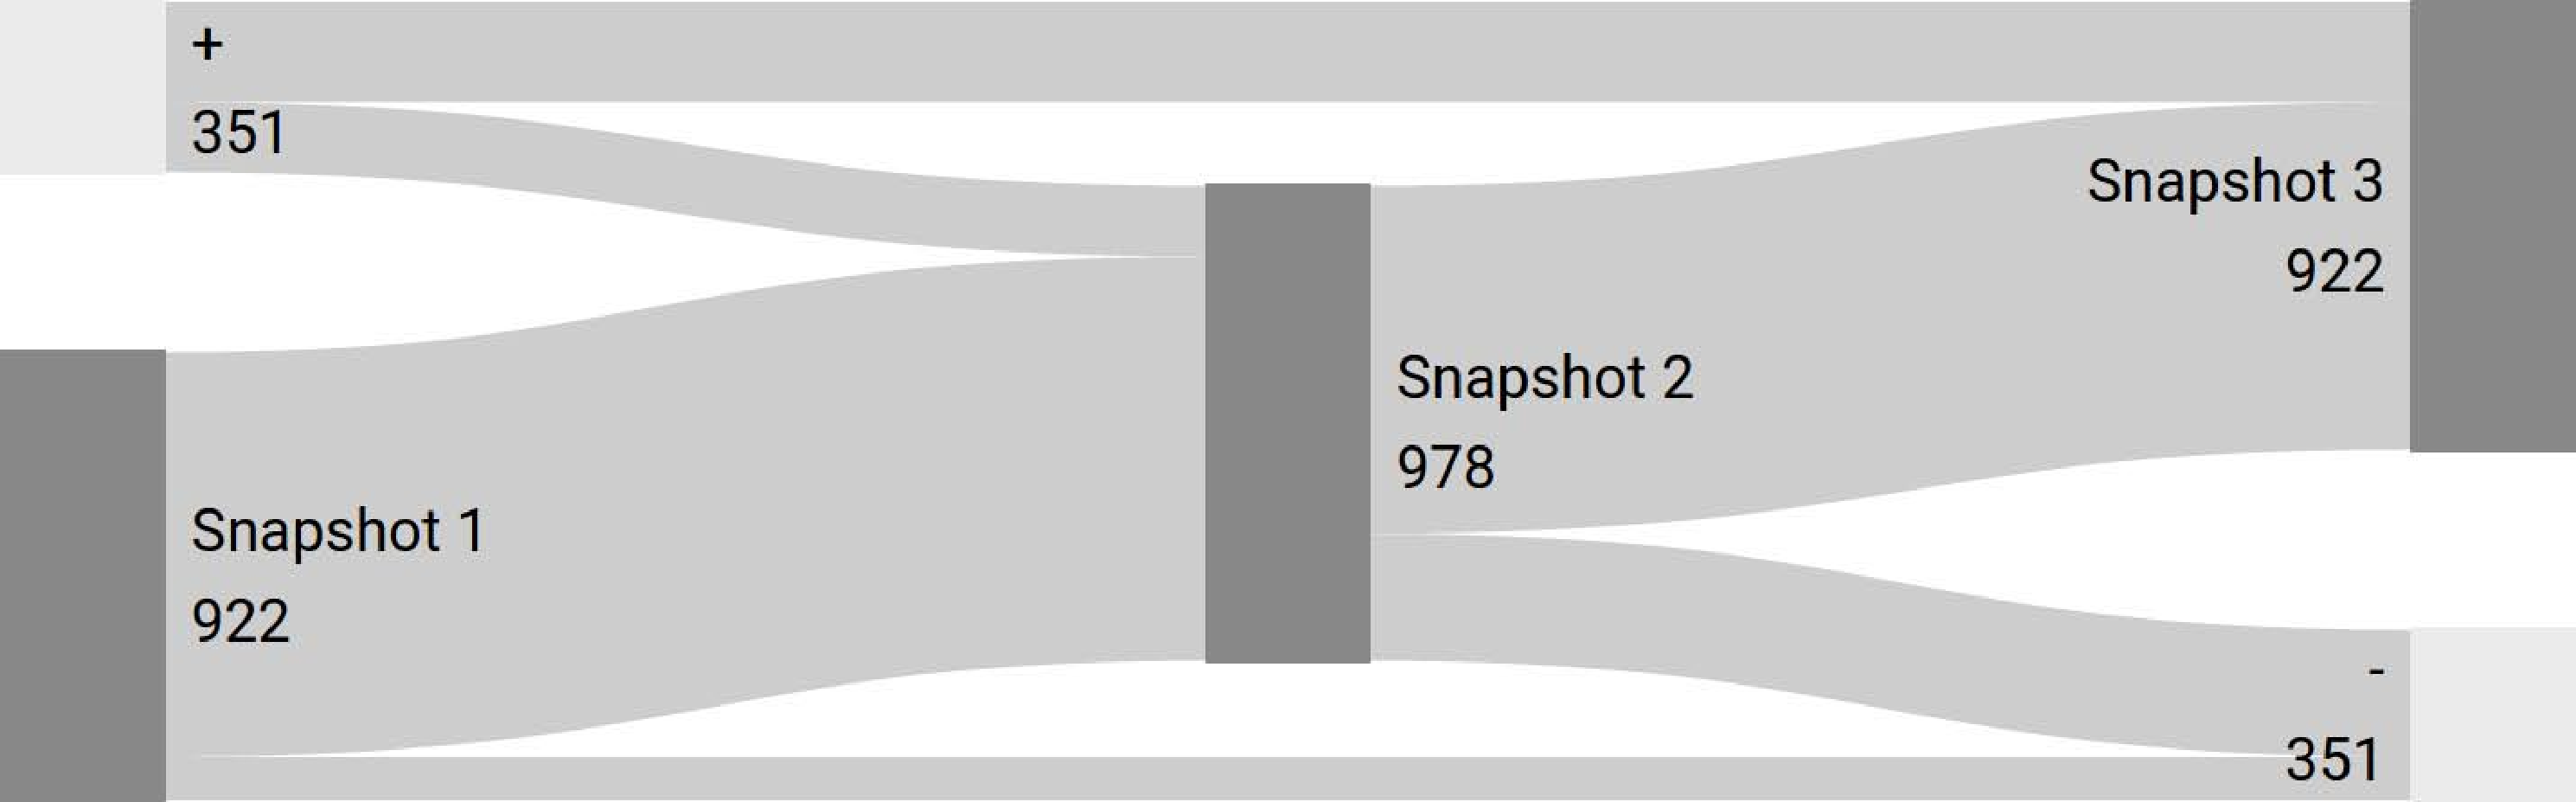
\includegraphics[width=.8\textwidth]{Figures/network_matching}
	\caption[Number of bees per snapshot]{\textbf{Number of bees per snapshot} This figure show the amount of bees for each snapshot and the proportion of intersecting.}
	\label{fig:network-matching}
\end{figure}

%%%%%%%%%%%%%%%%%%%%%%%%%%%%%%%%%%%%%%%%%%%%%%%%%%%%%%%%%%%%%%%%%%%%%%%%%%%%%%%
\subsection{Properties of the Bee Colony}
\label{subsec:colony}
%%%%%%%%%%%%%%%%%%%%%%%%%%%%%%%%%%%%%%%%%%%%%%%%%%%%%%%%%%%%%%%%%%%%%%%%%%%%%%%
Each snapshot consists of one component.
The density $D$ is over 50\% for all snapshots (69\%; 54\%; 61\%).
The diameter $\langle d_{\texttt{max}} \rangle$ is $3$ and the average shortest path length $\langle d \rangle$ is inbetween $1$ and $2$.
The global clustering coefficient $C_\Delta$ of all snapshots is higher than compared to an Erd\H{o}s-R\'{e}niy random graph, averaged over 100 runs using the same number of nodes and edges.
On average, each bee is connected to at least 50\% of the colony (68\%; 52\%; 61\%). During the ten hour observation peroid a bee interacts on average over $4,000$ times ($5,680$; $3,978$; $4,206$)
Table~\ref{tab:stats} summarizes those basic network properties for each snapshot and lists the values of its corresponding random graph.


Figure~\ref{fig:n3ageDist} shows the age distribution of the further investigated snapshot 3. This distribution corresponds to the artificial tagging of the bees. Consequently, bees of certain age groups are simply not present. The detection frequency of an individual bee is negatively correlated with its age (figure~\ref{fig:n3detfVSage}).

\begin{table}[htbp]
\small
\centering
\caption[Global network properties]{\textbf{Global network properties} $N$ number of nodes, $L$ number of links, $D$ diameter, $\langle d_{\texttt{max}} \rangle$ average path length, $\langle d \rangle$ diameter, $C_\Delta$ global clustering coefficient, $\langle k \rangle$ average degree and $\langle s \rangle$ represents the average strength, as introduced in section~\ref{sec:definitions}.}
\label{tab:stats}
\vspace*{5mm}
\begin{tabular}{rccccccccc}
\toprule
{} &  $N$ &   $L$ &  $D$ &  $\langle d_{\texttt{max}} \rangle$ &  $\langle d \rangle$ &   $C_\Delta$ & $\langle k \rangle$ &  $\langle s \rangle$ \\
\midrule
Snapshot 1 & 922 & 291179 & 0.69 & 3 & 1.32 &  0.79 & 631.62 & 5680.17 \\
Random 1  & 922 & 291179 & 0.69 & 2 & 1.31 &  0.69 & 631.62 & - \\ \midrule
Snapshot 2 & 978 & 256066 & 0.54 & 3 & 1.46 &  0.72 & 523.65 & 3977.94 \\
Random 2  & 978 & 256066 & 0.54 & 2 & 1.46 &  0.54 & 523.65 & - \\ \midrule
Snapshot 3 & 922 & 259421 & 0.61 & 3 & 1.39 &  0.75 & 562.74 & 4205.99 \\
Random 3  & 922 & 259421 & 0.61 & 2 & 1.39 &  0.61 & 562.74 & - \\
\bottomrule
\end{tabular}
\end{table}

The edge weight distribution is shown in figure~\ref{fig:edgeWdist}.
Most edges have a low weight; only a few edges have a high weight.
It seems that bees do not prefer individuals bees for interaction.[TODO. figure out what it means.]

\begin{figure}[bp]
	\centering
	\begin{subfigure}[b]{1\textwidth}
	\centering
	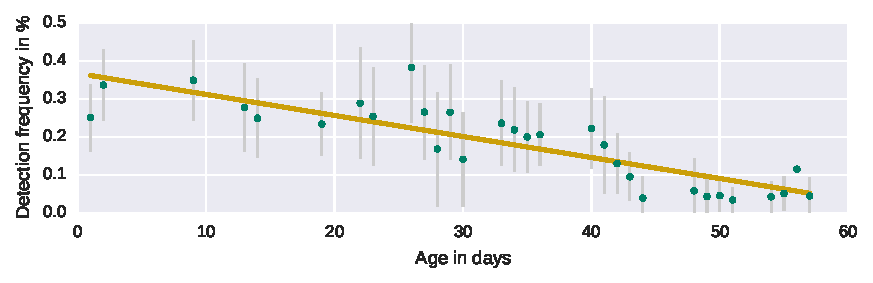
\includegraphics[width=1.0\textwidth]{Figures/n3_detFvsAge}
	\caption[Correlation]{Correlation}
	\label{fig:n3detfVSage}
	\end{subfigure} 
	\begin{subfigure}[b]{1\textwidth}
	\centering
	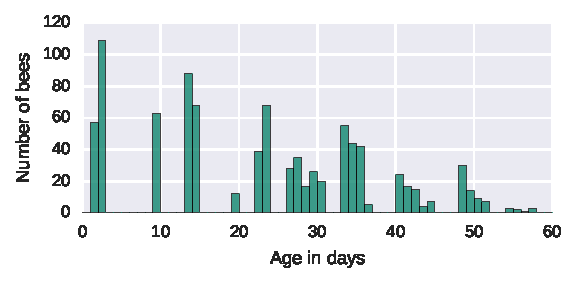
\includegraphics[width=1.0\textwidth]{Figures/n3_ages.pdf}
	\caption[Age distribution]{Age distribution}
	\label{fig:n3ageDist}
	\end{subfigure}
	\caption[Age distribution and correlation with detection frequency of snapshot~3]{\textbf{Age distribution and correlation with detection frequency of snapshot~3} (a) Detection frequency and the age of a bee seem to be negatively correlated. (b) The age of bees ranges from one to 60 day, but some age groups are missing.}
	\label{fig:ageDetF}
\end{figure}

\begin{figure}[htb]
	\begin{subfigure}[b]{0.49\textwidth}
	\centering
	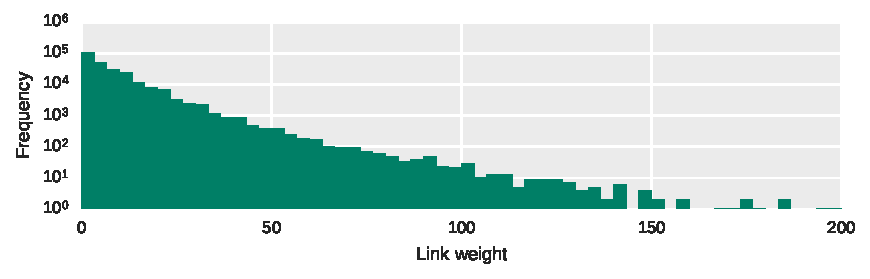
\includegraphics[width=1.0\textwidth]{Figures/n3-edgeWeightDist.pdf}
	\caption[Edge weight distribution]{Edge weight distribution}
	\label{fig:edgeWdist}
	\end{subfigure}
	\caption[Edge wights]{\textbf{Edge wights} (a) Correlation between number of interactions and total duration of interactions. The number of interactions is chose as the edge weight. (b)  The edge weight distribution decays exponentially.}
	\label{fig:edges}
\end{figure}
%%%%%%%%%%%%%%%%%%%%%%%%%%%%%%%%%%%%%%%%%%%%%%%%%%%%%%%%%%%%%%%%%%%%%%%%%%%%%%%
\subsection{Characteristics of Bees}
\label{subsubsec:bees}
%%%%%%%%%%%%%%%%%%%%%%%%%%%%%%%%%%%%%%%%%%%%%%%%%%%%%%%%%%%%%%%%%%%%%%%%%%%%%%%
For snapshot~3, I inspected the properties of each honey bee, concerning its degree~$k$, strength~$s$, local clustering coefficient~(lcc)~$c$, betweenness centrality~$C_B$ and closeness centrality~$C_C$ and derived charctersitics and properties of the honey bee colony.

\subsubsection{Low Hierarchical Structure}
The degree is normally distributed (a in figure~\ref{fig:n3-degreeStrLCC}).
Therefore most bees bee have the same high number of interaction partners.
The absence of hubs, a small number of highly connected bees, indicates a low hierarchical structure of the network.
Strength and lcc are also normally distributed (d and g in figure~\ref{fig:n3-degreeStrLCC}).
That also shows the absence of extreme values and confirms that bees are similar to each other regarding those properties.
Betweenness and closeness centrality (j and m in figure~\ref{fig:n3-degreeStrLCC}) also follow a normal distribution.
This leading to the assumption that no central or important bees exist.
All bees are similarly close to all other bees in the network, and every bee can reach any other bee with a few steps.
That also corresponds to the low average path length, and the small diameter of the network described in section~\ref{subsec:colony}.
The absence of bees with a high betweenness suggests that the colonies functionality is robust concerning the disappearance of single individuals.

\subsubsection{Local Network Measures and Detection Frequency}
Degree, strength, closeness and betweenness (b, e, k, and n in figure~\ref{fig:n3-degreeStrLCC}) show a positive correlated with the detection frequency. A low value corresponds to a low detection frequency. In contrast, the local clustering coefficient (h in figure~\ref{fig:n3-degreeStrLCC}) and detection frequency are negatively correlated.

\subsubsection{Local Network Measures and Age of Bees}
The histograms of degree, strength, betweenness, and closeness show a normal distribution with a tendency for bimodality. The local clustering coefficient distribution is instead right skewed, with one peak at $0.75$

There is no clear border between groups in the degree distribution plot (a), but a value around 0.4 can be estimated.
The strength histogram (d) seems to have a border at 1000.
For closeness (j) and betweenness (m), a border can be seen at 0.6 and 0.0001.
All distributions indicate a small group (~100 bees) and a second larger group containing the rest of the colony.

The first small group interacts on average with 20\% of the colony and has a very low strength (number of total interactions below 250). The closeness value is compared to the second group smaller but still over 0.5. The betweenness has a small range and is close to 0 for the first smaller group.
The second group interacts with about 80\%, corresponding to almost the entire colony and an average strength of 5000. A high strength can result from lots of neighbors with low edge weights or a few neighbors with high edge weight. The second is rather unlikely, looking at the edge weight distribution (figure~\ref{fig:edgeWdist}). The second group is characterized by a very high closeness (0.75) and a still very low betweenness but higher than the first group (0.0005).

All age-correlation plot show a seperate group of bees older than 45 days, seeming to correspond to the first smaller group of bees described above.
This older group is characterized by a low degree, a low strength, and low closeness and betweenness. In contrast, a high lcc, compared to the younger group is noticeable.
The younger group relates to a high degree and strength, as well as a high betweeness and closeness compared to the first group, but a lower lcc.
A high lcc of the old group indicates a high connectivity within the younger group and less connectivity between bees of the older group.

\begin{figure}[!h]
	\centering
	\begin{subfigure}[b]{1.0\textwidth}
	\centering
	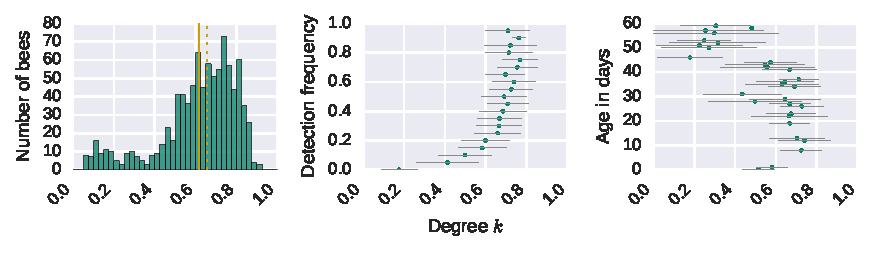
\includegraphics[width=1.0\textwidth]{Figures/n3-stat-degreeAgeDetF.pdf}
	%\caption[Degree]{\textbf{Degree}}
	%\label{fig:n3-degree}
	\end{subfigure}
	\begin{subfigure}[b]{1.0\textwidth}
	\centering
	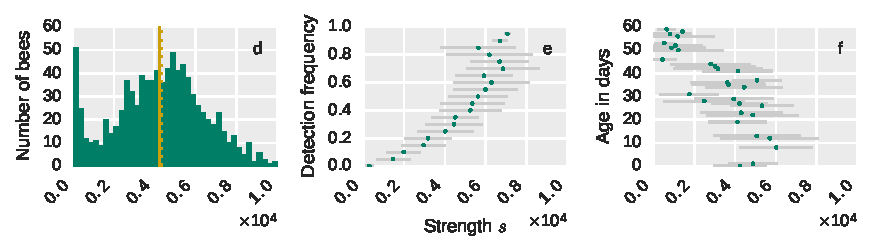
\includegraphics[width=1.0\textwidth]{Figures/n3-stat-strengthAgeDetF.pdf}
	%\caption[Strength]{\textbf{Strength}}
	%\label{fig:n3-strength}
	\end{subfigure}
	\begin{subfigure}[b]{1.0\textwidth}
	\centering
	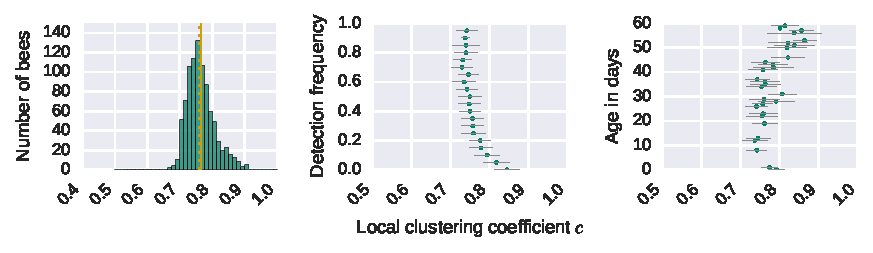
\includegraphics[width=1.0\textwidth]{Figures/n3-stat-lccAgeDetF.pdf}
	%\caption[Local clustering coefficient]{\textbf{Local clustering coefficient}}
	%\label{fig:n3-lcc}
	\end{subfigure}
	\begin{subfigure}[b]{1.0\textwidth}
	\centering
	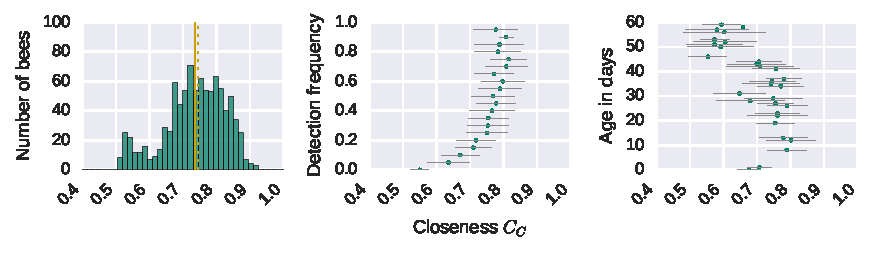
\includegraphics[width=1.0\textwidth]{Figures/n3-stat-closenessAgeDetF.pdf}
	%\caption[Closeness Centrality]{\textbf{Closeness Centrality}}
	%\label{fig:n3-closeness}
	\end{subfigure}
	\begin{subfigure}[b]{1.0\textwidth}
	\centering
	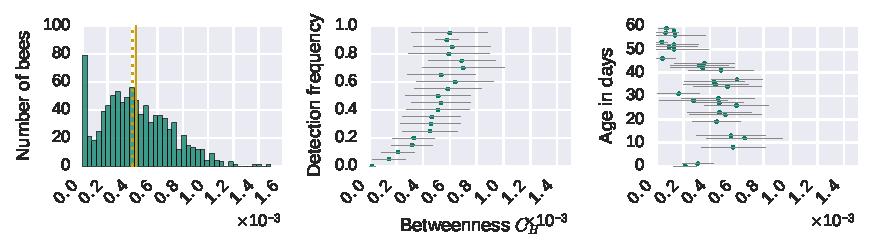
\includegraphics[width=1.0\textwidth]{Figures/n3-stat-betweenAgeDetF.pdf}
	%\caption[Betweeness Centrality]{\textbf{Betweeness Centrality}}
	%\label{fig:n3-between}
	\end{subfigure}
	\caption[Local measures in relation to age and detection frequency]{\textbf{Local measures in relation to age and detection frequency}}
	\label{fig:n3-degreeStrLCC}
\end{figure}
%%%%%%%%%%%%%%%%%%%%%%%%%%%%%%%%%%%%%%%%%%%%%%%%%%%%%%%%%%%%%%%%%%%%%%%%%%%%%%%
\subsection{Functional Groups within the Colony}
%%%%%%%%%%%%%%%%%%%%%%%%%%%%%%%%%%%%%%%%%%%%%%%%%%%%%%%%%%%%%%%%%%%%%%%%%%%%%%%

The leading eigenvector (LE) community detection algorithms revealed two communities with a similar size (modularity score of 0.25). The walktrap algorithm (WT) discovered three communities instead, also evenly distributed (modularity score of 0.23). Table~\ref{tab:n3-communities} lists the precise number of members per community and algorithm for snapshot~3.

For both algorithms the communities correspond to different age groups. For LE, the average age of the young community is $13.2$ days, and for the old community $28.7$ days. For WT, the average age of the young community is $6.6$ days and $29.3$ days for the older commmunity. The third middle-aged community of WT is on average 25.1 days old. The age distribution for each algorithm is represented in figure~\ref{fig:n3ageLE} and~\ref{fig:n3ageWT}. The two sample Kolmogorov-Smirnov test confirmed that the age distributions per community are significantly different. The corresponding $p$-values are listed in table~\ref{tab:n3-pvalues2}.

Each community occupies a different region of the comb.
Figure~\ref{fig:n3-communities} shows that the young communities spend the most time in the comb center and the old communities closer to the hive exit. The middle-aged community is positioned between the young and old community and in the periphery of the comb.

\begin{table}[htb]
\small
\centering
\caption[Communities per algorithm]{\textbf{Communities per algorithm} Communities marked with * contain the queen. Age and standard deviation (SD) are measured in days. The queen and nine bees with a negative age are excluded from this analysis.}
\label{tab:n3-communities}
\vspace*{5mm}
\begin{tabular}{lcrrrrr}
	\toprule
	{}  & Community ID & Members & Proportion & Age & SD\\
	\midrule  
	\quad LE  & CY & $*381$  & 41.78\% & $13.15$ & $\pm13.50$ \\
	          & CO & $531$   & 58.22\% & $28.70$ & $\pm11.67$ \\
    \midrule 
	\quad WT & CY & $*229$  & 25.11\% & $6.55$  & $\pm10.36$\\
			 & CM & $298$  & 32.68\% & $25.08$ & $\pm11.97$\\
			 & CO & $385$  & 42.21\% & $29.29$ & $\pm11.44$\\
	\bottomrule
\end{tabular}
\end{table}
\begin{table}[htb]
\small
\centering
\caption[Kolmogorov-Smirnov test]{\textbf{Kolmogorov-Smirnov test} $p$-values for leading eigenvector (LE) and walktrap (WT)}
\label{tab:n3-pvalues2}
\vspace*{5mm}
\begin{tabular}{crrrrr}
	\toprule
	 Communities & LE p-value & WT p-value\\
	\midrule 
    CY, CO & 5.10e-66 & 5.51e-67\\
    CY, CM &          & 1.10e-95\\
    CM, CO &          & 1.98e-05\\ 
	\bottomrule
\end{tabular}
\end{table}

\begin{figure}[!htb]
	\centering
	\begin{subfigure}[b]{1.0\textwidth}
	\centering
	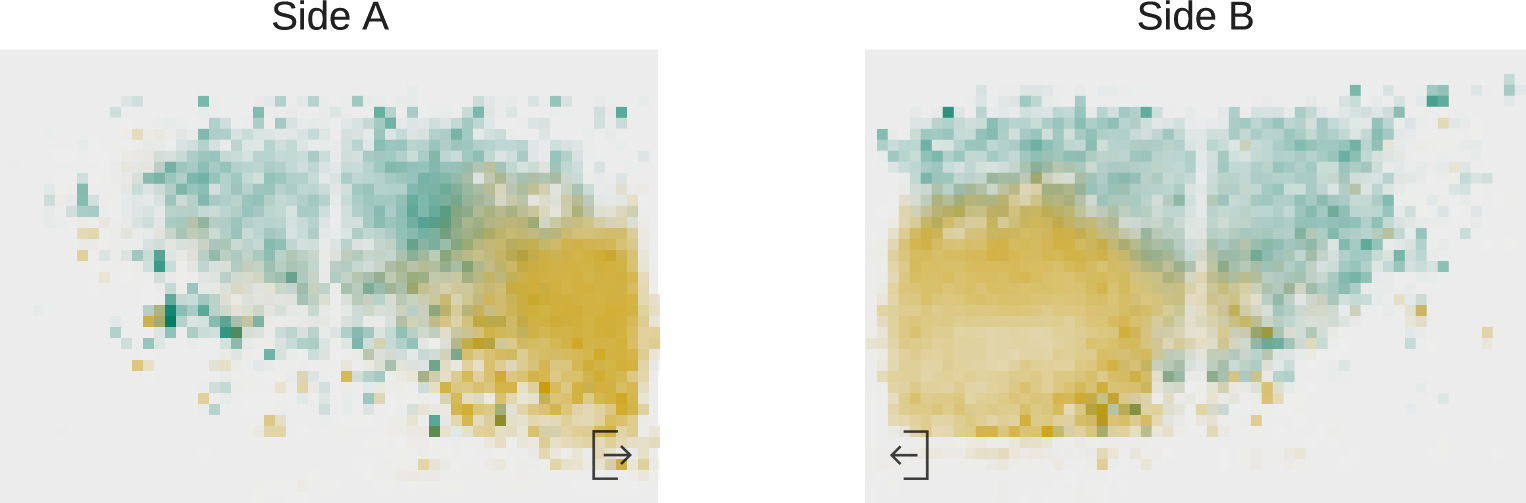
\includegraphics[width=1.0\textwidth]{Figures/le_network3}
	\end{subfigure}
	
	\begin{subfigure}[b]{1.0\textwidth}
	\centering
	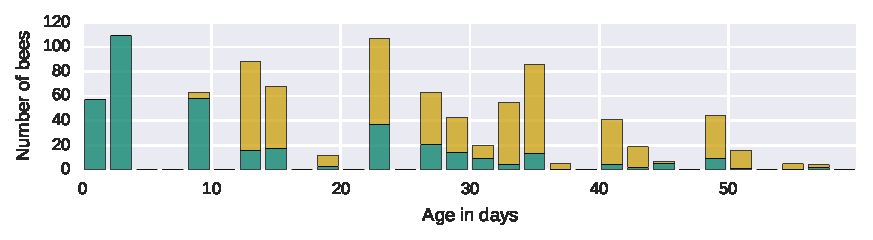
\includegraphics[width=1.0\textwidth]{Figures/n3-ageDistribution-LE}
	\caption[Leading eigenvector communities]{Leading eigenvector communities}
	\label{fig:n3ageLE}
	\end{subfigure}
	
	
	
	\begin{subfigure}[b]{1.0\textwidth}
	\vspace{1pt}
	\centering
	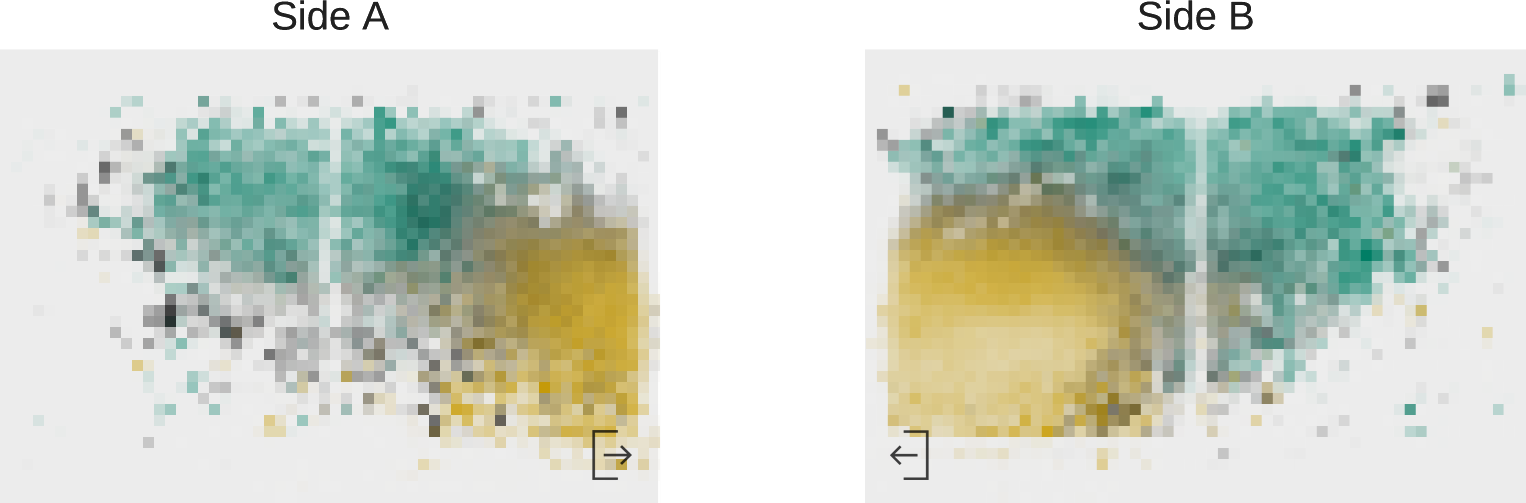
\includegraphics[width=1.0\textwidth]{Figures/wt_network3}
	\end{subfigure}
	
	\begin{subfigure}[b]{1.0\textwidth}
	\centering
	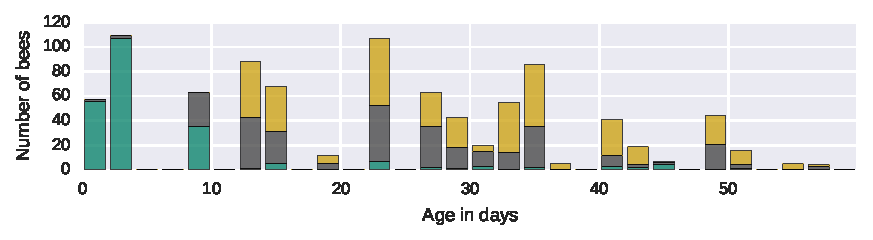
\includegraphics[width=1.0\textwidth]{Figures/n3-ageDistribution-WT}
	\caption[Walktrap communities]{Walktrap communities}
	\label{fig:n3ageWT}
	\end{subfigure}
	
	
	\caption[Age and spatial distribution of communities]{\textbf{Age and spatial distribution of communities} \emph{Green} represents the young community occupying the center area of the comb and \emph{orange} the old community, which is situated closer to the hive access. For walktrap the \emph{gray} middle-aged community is positioned between the other to and in the periphery of the comb.}
	\label{fig:n3-communities}
\end{figure}